\documentclass[11pt]{article}
\usepackage{graphicx}
\usepackage{amsmath}
\usepackage{amssymb}

% Margins
\topmargin=-0.45in
\evensidemargin=0in
\oddsidemargin=0in
\textwidth=6.5in
\textheight=9.0in
\headsep=0.25in

\title{
	\centering
	
\includegraphics[width=5cm]{univ-logo} \\
	\vspace{5cm}
	\textbf{SAT solvers} \\
	Computational Models of Argumentation
	\vspace{5cm}
}
\author{
    Christophe Yang \\
    Quentin Januel \\
    Sylvain Declercq
}
\date{2022}

\begin{document}

\maketitle
\newpage
\section{Rappel du projet}
L’argumentation abstraite [Dung 95] est un formalisme de raisonnement qui permet de representer des
informations contradictoires et d’en tirer des conclusions.
Un système d’argumentation est un graphe
dont les noeuds sont appelés arguments, et les arcs sont appelés attaques. La méthode de raisonnement
classique à partir de ces cadres argumentatifs est basée sur des sémantiques à extensions. Une extension
est un ensemble d’arguments qui représente une solution acceptable du problème d’argumentation. Avec
ce type de méthode de raisonnement, un argument peut avoir un statut accepté ou rejeté. Parmi les
méthodes de calcul les plus efficaces pour l’argumentation abstraite, une d’entre elles consiste à traduire
le problème en instance du problème SAT (ou d’un problème lié à SAT), et de résoudre ce nouveau
problème via un solveur SAT. De nombreux solveurs SAT existent, avec chacun leurs forces et leurs
faiblesses, qui peuvent varier selon la nature des instances à résoudre. Des études récentes [Gning and
Mailly 2020, Klein and Thimm 2020] ont montré que changer le solveur SAT tout en conservant le même
encodage logique peut faire varier l’efficacité de l’approche.
\bigbreak
Nous souhaitons tester une approche ”portfolio” pour résoudre ce problème, c’est-à-dire développer un
solveur d’argumentation qui traduit le problème à résoudre en instance de SAT, et qui utilise une
combinaison de plusieurs solveurs SAT pour tenter de le résoudre. Il est possible d’effectuer un prétraitement 
pour identifier quel solveur SAT est le plus indiqué en fonction de l’instance (ce qui nécessite
une étude préliminaire pour associer à chaque type de système d'argumentation son solveur SAT). Une
autre approche possible consiste à exécuter en parallèle tous les solveurs SAT à disposition, et d’arrêter le
calcul lorsqu’un des solveurs a trouvé la solution. L’inconvénient de cette approche est que son efficacité
est grandement liée au nombre de processeurs/coeurs de calcul disponibles.
Une fois une (ces) méthode(s) implémentée(s), son (leur) efficacité sera évaluée notamment grâce aux
systèmes d’argumentation utilisés dans le cadre des compétitions de solveurs d’argumentation ICCMA
[Thimm and Villata 2017, Gaggle et al 2019].

\section{Implémentation d'un système d'argumentation abstraite}
Le langage de programmation utilisé pour l'implémentation est Rust.\\
Au début du projet, nous représentions les graphes comme étant un liste d'arguments (sous forme de string) \\
et une liste d'attaques (tuples de strings, le premier est l'attaquant et le deuxième l'attaqué).\\
Cepedant nous avons remarquer que cette structure de données ralentissais la traduction du problème en instance sat.\\
Nous avons donc rechercher à optimiser ce point là.\\
Nous représentons désormais la liste d'adjacence comme structure de données pour représenter notre graphe.\\
C'est une liste d'arguments mais chaque argument contient également ceux qui l'attaquent\\
(sous forme d'entier qui représentent l'indexe de l'attaquant dans la liste des arguments).
\section{Traduction du problème en instance du problème SAT}
Pour la traduction du problème en instance de problème SAT nous nous sommes inspirés du solver Coquiaas.\cite{lagniez2015coquiaas}\\

\section{Implémentation solveurs SAT}
Nous avons actuellement rajouter à notre portofolio de solveurs :
\begin{itemize}
	\item manysat
	\item glucose-pre (Avec prétraitement)
	\item glucose (Sans prétraitement)
	\item dpll (solveur fait maison)
	\item minisat
\end{itemize}

Ces solveurs peuvent être lancés en parallèle même si pour le moment nous ne le faisons pas.
\section{Générateur de graphes}
Nous avons créer des générateurs de graphes pour ces semantiques à l'aide \cite{arg2017Generator}:
\begin{itemize}
	\item grounded
	\item scc
	\item stable
\end{itemize}
\section{Benchmarks}

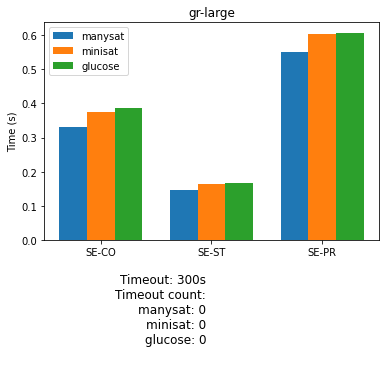
\includegraphics[scale=0.75]{img/gr-large.png}\\
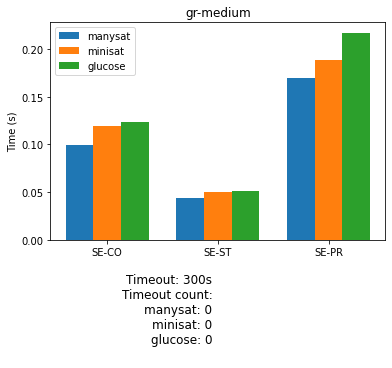
\includegraphics[scale=0.75]{img/gr-medium.png}\\
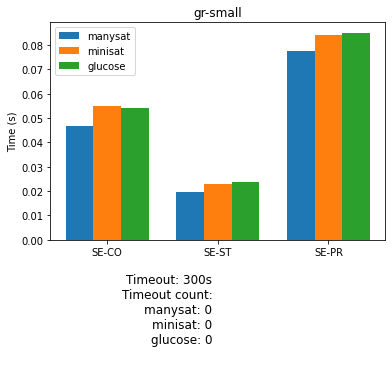
\includegraphics[scale=0.75]{img/gr-small.png}

% Bibliography
\bibliographystyle{ieeetr}
\bibliography{./citations}

\end{document}
